

\tikzset{every picture/.style={line width=0.75pt}} %set default line width to 0.75pt        

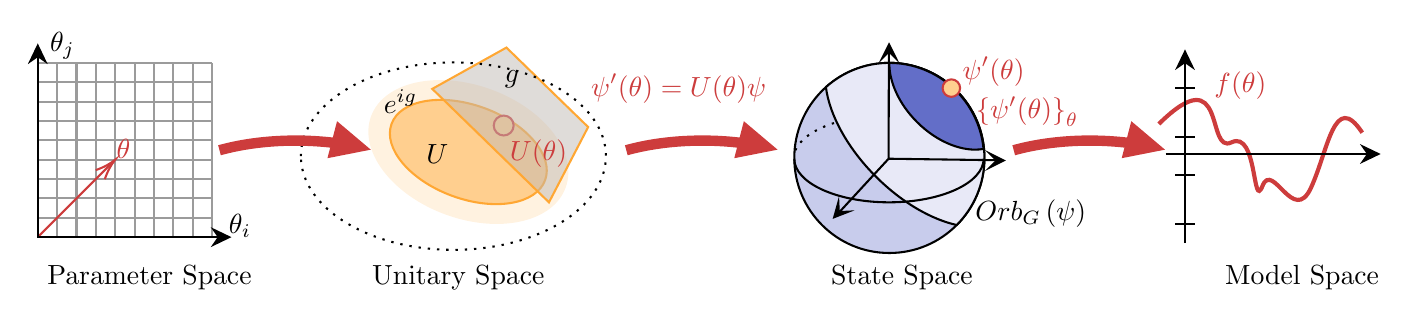
\begin{tikzpicture}[x=0.7pt,y=0.7pt,yscale=-1,xscale=1]
%uncomment if require: \path (0,137); %set diagram left start at 0, and has height of 137

%Curve Lines [id:da21159432878884543] 
\draw [color={rgb, 255:red, 205; green, 60; blue, 60 }  ,draw opacity=1 ][line width=1.5]    (584.72,49.37) .. controls (620.22,14.37) and (608.72,65.37) .. (622.22,58.87) .. controls (635.72,52.37) and (632.97,94.62) .. (638.22,81.37) .. controls (643.47,68.12) and (654.22,101.87) .. (663.22,82.37) .. controls (672.22,62.87) and (675.22,31.87) .. (689.72,53.87) ;
%Shape: Ellipse [id:dp8507927161982255] 
\draw  [draw opacity=0][fill={rgb, 255:red, 255; green, 242; blue, 224 }  ,fill opacity=1 ] (178.03,45.45) .. controls (184.55,27.64) and (212.33,21.43) .. (240.07,31.59) .. controls (267.82,41.74) and (285.02,64.42) .. (278.49,82.24) .. controls (271.97,100.05) and (244.19,106.26) .. (216.45,96.1) .. controls (188.71,85.94) and (171.51,63.27) .. (178.03,45.45) -- cycle ;
%Shape: Ellipse [id:dp04645940013130723] 
\draw  [color={rgb, 255:red, 255; green, 167; blue, 51 }  ,draw opacity=1 ][fill={rgb, 255:red, 255; green, 207; blue, 143 }  ,fill opacity=1 ] (188.63,49.33) .. controls (193.21,36.82) and (214.66,33.18) .. (236.56,41.19) .. controls (258.45,49.21) and (272.48,65.85) .. (267.9,78.36) .. controls (263.32,90.86) and (241.86,94.51) .. (219.97,86.49) .. controls (198.08,78.48) and (184.05,61.84) .. (188.63,49.33) -- cycle ;
%Shape: Ellipse [id:dp8227321930180724] 
\draw  [color={rgb, 255:red, 205; green, 60; blue, 60 }  ,draw opacity=1 ][fill={rgb, 255:red, 255; green, 207; blue, 143 }  ,fill opacity=1 ][line width=0.75]  (241.38,50.17) .. controls (241.38,47.33) and (243.68,45.03) .. (246.52,45.03) .. controls (249.36,45.03) and (251.66,47.33) .. (251.66,50.17) .. controls (251.66,53.01) and (249.36,55.31) .. (246.52,55.31) .. controls (243.68,55.31) and (241.38,53.01) .. (241.38,50.17) -- cycle ;
%Shape: Trapezoid [id:dp46205842243935824] 
\draw  [color={rgb, 255:red, 255; green, 167; blue, 51 }  ,draw opacity=1 ][fill={rgb, 255:red, 192; green, 185; blue, 179 }  ,fill opacity=0.5 ] (209.65,31.26) -- (247.93,9.94) -- (290.12,50.96) -- (269.89,89.83) -- cycle ;
%Shape: Ellipse [id:dp7235006458899723] 
\draw  [dash pattern={on 0.84pt off 2.51pt}] (141.83,65.98) .. controls (141.83,39.27) and (177.08,17.61) .. (220.56,17.61) .. controls (264.04,17.61) and (299.29,39.27) .. (299.29,65.98) .. controls (299.29,92.7) and (264.04,114.35) .. (220.56,114.35) .. controls (177.08,114.35) and (141.83,92.7) .. (141.83,65.98) -- cycle ;
%Shape: Ellipse [id:dp21567764947895118] 
\draw  [color={rgb, 255:red, 0; green, 0; blue, 0 }  ,draw opacity=1 ][fill={rgb, 255:red, 200; green, 204; blue, 236 }  ,fill opacity=1 ] (396.53,66.91) .. controls (396.53,39.81) and (418.5,17.84) .. (445.61,17.84) .. controls (472.71,17.84) and (494.68,39.81) .. (494.68,66.91) .. controls (494.68,94.01) and (472.71,115.98) .. (445.61,115.98) .. controls (418.5,115.98) and (396.53,94.01) .. (396.53,66.91) -- cycle ;
%Shape: Arc [id:dp8328098685967941] 
\draw  [draw opacity=0][dash pattern={on 0.84pt off 2.51pt}] (397.04,62.98) .. controls (401.44,52.62) and (421.33,44.8) .. (445.21,44.8) .. controls (472.31,44.8) and (494.28,54.88) .. (494.28,67.31) -- (445.21,67.31) -- cycle ; \draw  [dash pattern={on 0.84pt off 2.51pt}] (397.04,62.98) .. controls (401.44,52.62) and (421.33,44.8) .. (445.21,44.8) .. controls (472.31,44.8) and (494.28,54.88) .. (494.28,67.31) ;  
\draw  [fill={rgb, 255:red, 0; green, 0; blue, 0 }  ,fill opacity=1 ] (497.55,64.74) -- (504.56,68.24) -- (497.55,71.75) -- (501.06,68.24) -- cycle ;
\draw  [fill={rgb, 255:red, 0; green, 0; blue, 0 }  ,fill opacity=1 ] (441.93,15.43) -- (445.44,8.42) -- (448.94,15.43) -- (445.44,11.93) -- cycle ;
\draw  [fill={rgb, 255:red, 0; green, 0; blue, 0 }  ,fill opacity=1 ] (424.45,94.64) -- (417.15,97.48) -- (419.26,89.93) -- (419.5,94.88) -- cycle ;
%Curve Lines [id:da40312129843366473] 
\draw [color={rgb, 255:red, 205; green, 60; blue, 60 }  ,draw opacity=1 ][line width=3.75]    (309.81,62.94) .. controls (331.4,56.93) and (358.22,56.39) .. (381.2,61.09) ;
\draw [shift={(387.9,62.64)}, rotate = 194.53] [fill={rgb, 255:red, 205; green, 60; blue, 60 }  ,fill opacity=1 ][line width=0.08]  [draw opacity=0] (20.54,-9.87) -- (0,0) -- (20.54,9.87) -- cycle    ;
%Shape: Path Data [id:dp6682050236909869] 
\draw  [color={rgb, 255:red, 0; green, 0; blue, 0 }  ,draw opacity=1 ][fill={rgb, 255:red, 232; green, 233; blue, 247 }  ,fill opacity=1 ] (445.61,17.84) .. controls (472.71,17.84) and (494.68,39.81) .. (494.68,66.91) .. controls (494.68,80.42) and (489.22,92.66) .. (480.38,101.54) .. controls (467.18,98.59) and (451.98,89.87) .. (438.64,76.53) .. controls (423.78,61.67) and (414.66,44.5) .. (412.85,30.37) .. controls (421.53,22.58) and (433.02,17.84) .. (445.61,17.84) -- cycle ;
%Shape: Path Data [id:dp872501599073626] 
\draw  [color={rgb, 255:red, 0; green, 0; blue, 0 }  ,draw opacity=1 ][fill={rgb, 255:red, 99; green, 110; blue, 200 }  ,fill opacity=1 ] (459.87,48.36) .. controls (450.45,38.94) and (445.42,27.42) .. (445.61,17.84) .. controls (471.03,17.96) and (491.88,37.41) .. (494.22,62.25) .. controls (484,64.1) and (470.58,59.07) .. (459.87,48.36) -- cycle ;
%Shape: Ellipse [id:dp41350603939954467] 
\draw  [color={rgb, 255:red, 205; green, 60; blue, 60 }  ,draw opacity=1 ][fill={rgb, 255:red, 255; green, 207; blue, 143 }  ,fill opacity=1 ] (473.09,30.85) .. controls (473.09,28.36) and (475.11,26.34) .. (477.61,26.34) .. controls (480.1,26.34) and (482.13,28.36) .. (482.13,30.85) .. controls (482.13,33.35) and (480.1,35.37) .. (477.61,35.37) .. controls (475.11,35.37) and (473.09,33.35) .. (473.09,30.85) -- cycle ;
%Straight Lines [id:da7896640456924652] 
\draw    (445.21,67.31) -- (445.36,12.63) -- (445.21,67.31) -- (445.21,67.31) -- (419.5,95.2) -- (445.21,67.31) -- (501.13,68.09) ;
%Shape: Arc [id:dp9230931498609308] 
\draw  [draw opacity=0] (494.28,67.31) .. controls (494.28,67.31) and (494.28,67.31) .. (494.28,67.31) .. controls (494.28,67.31) and (494.28,67.31) .. (494.28,67.31) .. controls (494.28,79.74) and (472.4,89.82) .. (445.41,89.82) .. controls (418.41,89.82) and (396.53,79.74) .. (396.53,67.31) -- (445.41,67.31) -- cycle ; \draw   (494.28,67.31) .. controls (494.28,67.31) and (494.28,67.31) .. (494.28,67.31) .. controls (494.28,67.31) and (494.28,67.31) .. (494.28,67.31) .. controls (494.28,79.74) and (472.4,89.82) .. (445.41,89.82) .. controls (418.41,89.82) and (396.53,79.74) .. (396.53,67.31) ;  
%Shape: Grid [id:dp9617628915465708] 
\draw  [draw opacity=0] (96,17.8) -- (96,107.8) -- (6,107.8) -- (6,17.8) -- cycle ; \draw  [color={rgb, 255:red, 155; green, 155; blue, 155 }  ,draw opacity=1 ] (96,17.8) -- (6,17.8)(96,27.8) -- (6,27.8)(96,37.8) -- (6,37.8)(96,47.8) -- (6,47.8)(96,57.8) -- (6,57.8)(96,67.8) -- (6,67.8)(96,77.8) -- (6,77.8)(96,87.8) -- (6,87.8)(96,97.8) -- (6,97.8) ; \draw  [color={rgb, 255:red, 155; green, 155; blue, 155 }  ,draw opacity=1 ] (96,17.8) -- (96,107.8)(86,17.8) -- (86,107.8)(76,17.8) -- (76,107.8)(66,17.8) -- (66,107.8)(56,17.8) -- (56,107.8)(46,17.8) -- (46,107.8)(36,17.8) -- (36,107.8)(26,17.8) -- (26,107.8)(16,17.8) -- (16,107.8) ; \draw  [color={rgb, 255:red, 155; green, 155; blue, 155 }  ,draw opacity=1 ]  ;
%Straight Lines [id:da5913820732631816] 
\draw [color={rgb, 255:red, 205; green, 60; blue, 60 }  ,draw opacity=1 ]   (6,107.8) -- (44.59,69.21) ;
\draw [shift={(46,67.8)}, rotate = 135] [color={rgb, 255:red, 205; green, 60; blue, 60 }  ,draw opacity=1 ][line width=0.75]    (10.93,-3.29) .. controls (6.95,-1.4) and (3.31,-0.3) .. (0,0) .. controls (3.31,0.3) and (6.95,1.4) .. (10.93,3.29)   ;
%Straight Lines [id:da227565169944973] 
\draw    (103,107.8) -- (6,107.8) -- (6,10.8) ;
\draw [shift={(6,7.8)}, rotate = 90] [fill={rgb, 255:red, 0; green, 0; blue, 0 }  ][line width=0.08]  [draw opacity=0] (10.72,-5.15) -- (0,0) -- (10.72,5.15) -- (7.12,0) -- cycle    ;
\draw [shift={(106,107.8)}, rotate = 180] [fill={rgb, 255:red, 0; green, 0; blue, 0 }  ][line width=0.08]  [draw opacity=0] (10.72,-5.15) -- (0,0) -- (10.72,5.15) -- (7.12,0) -- cycle    ;
%Curve Lines [id:da7450089287440076] 
\draw [color={rgb, 255:red, 205; green, 60; blue, 60 }  ,draw opacity=1 ][line width=3.75]    (99.81,62.94) .. controls (121.4,56.93) and (148.22,56.39) .. (171.2,61.09) ;
\draw [shift={(177.9,62.64)}, rotate = 194.53] [fill={rgb, 255:red, 205; green, 60; blue, 60 }  ,fill opacity=1 ][line width=0.08]  [draw opacity=0] (20.54,-9.87) -- (0,0) -- (20.54,9.87) -- cycle    ;
%Curve Lines [id:da24180358408082503] 
\draw [color={rgb, 255:red, 205; green, 60; blue, 60 }  ,draw opacity=1 ][line width=3.75]    (509.81,62.94) .. controls (531.4,56.93) and (558.22,56.39) .. (581.2,61.09) ;
\draw [shift={(587.9,62.64)}, rotate = 194.53] [fill={rgb, 255:red, 205; green, 60; blue, 60 }  ,fill opacity=1 ][line width=0.08]  [draw opacity=0] (20.54,-9.87) -- (0,0) -- (20.54,9.87) -- cycle    ;
%Straight Lines [id:da409045524065621] 
\draw    (598.22,110.87) -- (598.22,13.87) ;
\draw [shift={(598.22,10.87)}, rotate = 90] [fill={rgb, 255:red, 0; green, 0; blue, 0 }  ][line width=0.08]  [draw opacity=0] (10.72,-5.15) -- (0,0) -- (10.72,5.15) -- (7.12,0) -- cycle    ;
%Straight Lines [id:da24996380649955274] 
\draw    (588.22,64.87) -- (696.22,64.87) ;
\draw [shift={(699.22,64.87)}, rotate = 180] [fill={rgb, 255:red, 0; green, 0; blue, 0 }  ][line width=0.08]  [draw opacity=0] (10.72,-5.15) -- (0,0) -- (10.72,5.15) -- (7.12,0) -- cycle    ;
%Straight Lines [id:da7522987321356736] 
\draw    (593.22,55.87) -- (603.22,55.87) ;
%Straight Lines [id:da957047975933722] 
\draw    (593.22,30.87) -- (603.22,30.87) ;
%Straight Lines [id:da38309824074191656] 
\draw    (593.22,75.87) -- (603.22,75.87) ;
%Straight Lines [id:da4790769801983854] 
\draw    (593.22,100.87) -- (603.22,100.87) ;

% Text Node
\draw (248.1,55.84) node [anchor=north west][inner sep=0.75pt]  [font=\normalsize,color={rgb, 255:red, 205; green, 60; blue, 60 }  ,opacity=1 ] [align=left] {$\displaystyle \textcolor[rgb]{0.80,0.24,0.24}{U}\textcolor[rgb]{0.80,0.24,0.24}{(}\textcolor[rgb]{0.80,0.24,0.24}{\theta }\textcolor[rgb]{0.80,0.24,0.24}{)}$};
% Text Node
\draw (183.0,30.0) node [anchor=north west][inner sep=0.75pt]  [font=\normalsize] [align=left] {$\displaystyle e^{i\mathfrak{g}}$};
% Text Node
\draw (205.0,58.23) node [anchor=north west][inner sep=0.75pt]  [font=\normalsize] [align=left] {$\displaystyle \mathbb{U}$};
% Text Node
\draw (290.0,22.00) node [anchor=north west][inner sep=0.75pt]  [font=\normalsize] [align=left] {$\displaystyle \textcolor[rgb]{0.80,0.24,0.24}{\ket{\psi '( \theta )}= U (\theta) \ket{\psi}}$};
% Text Node
\draw (481.84,13.18) node [anchor=north west][inner sep=0.75pt]  [font=\normalsize,color={rgb, 255:red, 205; green, 60; blue, 60 }  ,opacity=1 ] [align=left] {$\displaystyle \ket{\psi '( \theta )}$};
% Text Node
\draw (245.47,20.08) node [anchor=north west][inner sep=0.75pt]  [font=\normalsize] [align=left] {$\displaystyle \mathfrak{g}$};
% Text Node
\draw (488.45,86.63) node [anchor=north west][inner sep=0.75pt]  [font=\normalsize] [align=left] {$\displaystyle \text{Orb}_{G}\left(\ket{\psi }\right)$};
% Text Node
\draw (488.84,33.5) node [anchor=north west][inner sep=0.75pt]  [font=\normalsize,color={rgb, 255:red, 205; green, 60; blue, 60 }  ,opacity=1 ] [align=left] {$\displaystyle \left\{\ket{\psi '( \theta )}\right\}_{\theta }$};
% Text Node
\draw (103.0,94.41) node [anchor=north west][inner sep=0.75pt]  [font=\normalsize] [align=left] {$\displaystyle \theta _{i}$};
% Text Node
\draw (10.8,0.2) node [anchor=north west][inner sep=0.75pt]  [font=\normalsize] [align=left] {$\displaystyle \theta _{j}$};
% Text Node
\draw (45.1,55.84) node [anchor=north west][inner sep=0.75pt]  [font=\normalsize,color={rgb, 255:red, 205; green, 60; blue, 60 }  ,opacity=1 ] [align=left] {$\displaystyle \theta $};
% Text Node
\draw (611.84,21) node [anchor=north west][inner sep=0.75pt]  [font=\normalsize,color={rgb, 255:red, 205; green, 60; blue, 60 }  ,opacity=1 ] [align=left] {$\displaystyle f( \theta )$};
% Text Node
\draw (9.33,120.67) node [anchor=north west][inner sep=0.75pt]  [font=\rmfamily] [align=left] {Parameter Space};
% Text Node
\draw (177,120.8) node [anchor=north west][inner sep=0.75pt]  [font=\rmfamily] [align=left] {Unitary Space};
% Text Node
\draw (414,120.8) node [anchor=north west][inner sep=0.75pt]  [font=\rmfamily] [align=left] {State Space};
% Text Node
\draw (617.39,120.8) node [anchor=north west][inner sep=0.75pt]  [font=\rmfamily] [align=left] {Model Space};


\end{tikzpicture}
